\section{Background}
\label{sec-motivation}

%\fixme{I changed section2 title to Background}
%Our work focuses mainly on switches supporting the popular
%OpenFlow~\cite{openflow} protocol, specifically OpenFlow 1.0, which is
%widely available in production switches today. As we will be clear,
%our results apply qualitatively to more recent versions of OpenFlow
%e.g., OpenFlow 1.3., as well.

%\subsection{Basics}
Instead of running a complex control plane on each switch, SDN delegates
network control to external applications running on a logically central
controller. 
%In SDN, network control is delegated to external applications running on a
%logically central controller, rather than running a complex control plane on
%each switch. 
Applications determine the routes traffic should take, and they
instruct the controller to update switches with the appropriate forwarding
state. These decisions may be based on data packets that are
received by switches and sent to the controller. Such packet events and
state update operations are enabled by OpenFlow~\cite{openflow}---a standard
API implemented by switches to facilitate communication with the controller.
%An SDN switch by default does not run control plane protocols, as these are
%delegated to an external application running on a logically central
%controller. Applications determine the routes traffic must take through the
%network and instruct the controller to update the switching substrate with
%the appropriate forwarding state. OpenFlow~\cite{openflow} is a widely
%adopted SDN API employed by switches to communicate with the controller to
%enable such state update operations. 
Although SDN moves control plane logic from switches to a central controller, 
switches must still perform several steps to generate packet events and update
forwarding state. We describe these steps below.
%; we articulate these steps below. 
%\fixme{I cut the sentence after here}
%We then highlight several
%applications whose efficacy is heavily impacted by the latency of these
%control operations on switches. 

% The next section discusses our measurements
% of these latencies, and shows that the root causes of latency are unlikely
% to be eliminated without substantial changes in switch hardware, OpenFlow
% specifications, or control application design.

%\subsection{Components of Latency}

\begin{figure}
\centering
%%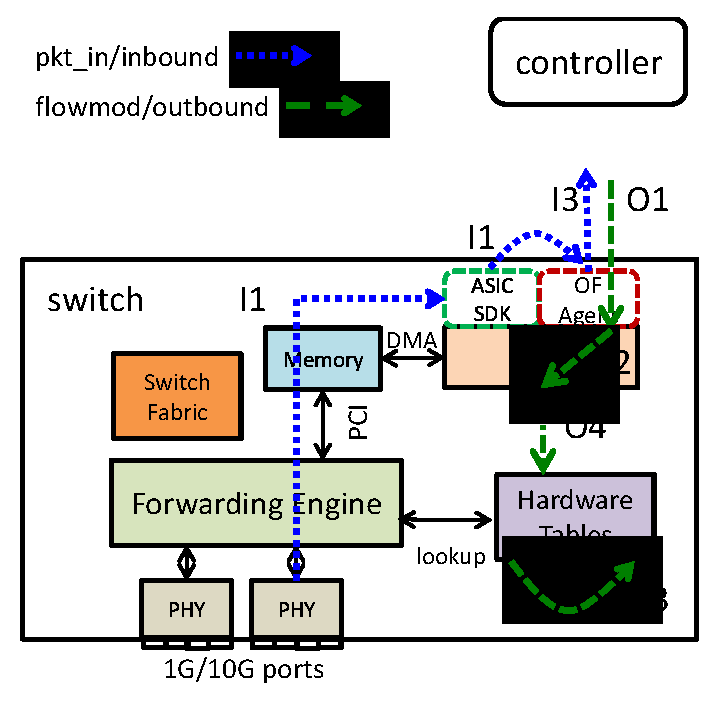
\epsfig{file=./figs/openflow_switch_illustrate.eps,width=0.4\textwidth} %%changed
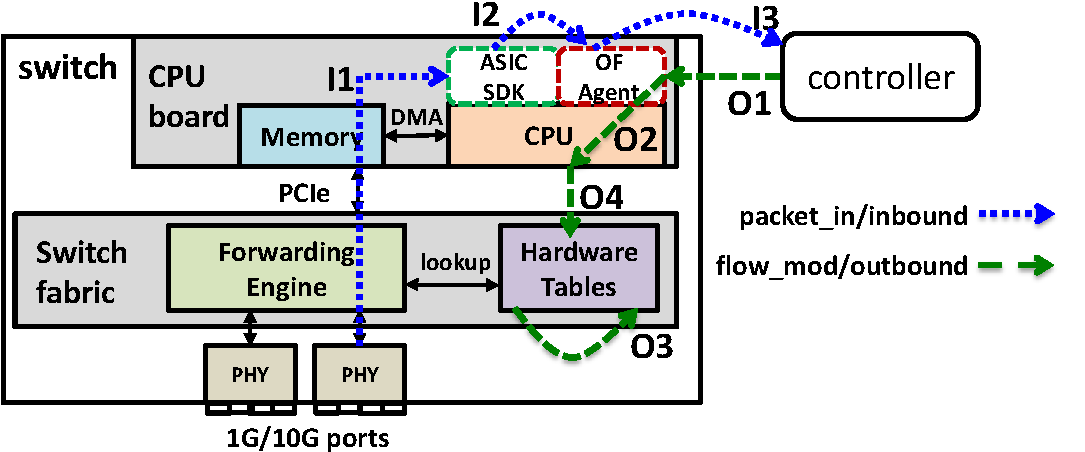
\includegraphics[width=0.98\columnwidth]{figs/openflow_switch.pdf}
\compactcaption{Schematic of an OpenFlow switch. 
%Different rectangular blocks indicate different components of a switch; 
%different boxes do not mean different chips. 
We also show the factors contributing to inbound and outbound latency}\label{openflow_switch_delay}
%\vspace{-0.05in}
\end{figure}

\minisection{Packet Arrival} When a packet arrives, the switch ASIC first
performs a lookup in the switch's hardware forwarding tables. If a match is
found, the packet is forwarded at line rate. Otherwise the following steps
occur (Figure~\ref{openflow_switch_delay}): (I1) The ASIC sends the packet to the switch's CPU via the PCIe bus. (I2) An OS
interrupt is raised, at which point the ASIC SDK gets the packet and
dispatches it to the switch-side OpenFlow agent. (I3) The agent wakes up,
processes the packet, and sends to the controller a \packetin message
containing metadata and the first 128B of the packet. All three steps,
I1--I3, can impact the latency in generating a \packetin message. We
categorize this as {\em inbound latency}, since the controller receives the
message as input.

\minisection{Forwarding Table Updates} 
\iffalse
The application residing on the controller
processes the \packetin, and upon determining a route for packets
belonging to the corresponding flow, sends a \flowmod message and a \packetout
message. \flowmod can also be sent by a controller without receiving a \packetin.

A \flowmod message describes the action the switch should apply to
all future packets of the flow: this could be forward according to some rule,
update an existing rule, or delete a rule. The format of a ``simple''
wildcard rule is \emph{inport=1,dstip=10.0.0.2,action=output:3}.\footnote{In
OpenFlow 1.0, a rule can match up to 12 common header fields.}
The rule may also specify a priority (to determine which rule to apply when
multiple rules match a packet) and a timeout after which the rule is deleted
from the table. 
\fi
The controller sends \flowmod messages to update a
switch's forwarding tables.
A switch takes the following steps to handle a \flowmod
(Figure~\ref{openflow_switch_delay}): (O1) The
OpenFlow agent running on the CPU parses the message. (O2) The agent
schedules the addition (or removal) of the forwarding rule in hardware tables, typically TCAM.  (O3)
Depending on the nature of the rule, the chip SDK may require existing rules
in the tables to be rearranged, e.g., to accommodate high priority rules.
(O4) The rule is inserted (or removed) in the hardware table.  All four steps, O1--O4,
impact the total latency in executing a \flowmod action. We categorize this
as {\em outbound latency}, since the controller outputs a \flowmod message.

\iffalse
A \packetout message releases a specific packet buffered at the switch, and
the switch forwards it as specified in the message. The steps taken by the
switch are the inverse of those for generating \packetin messages; the
latency for these steps is another form of {\em outbound latency}.
\fi

% The actions described above are generally applicable to different
% versions of OpenFlow. \aditya{correct? do we need to say more?}

% In this paper, we focus on the delays imposed at the switch. We ignore
% the impact of the propagation delay to the controller and control
% application processing itself. The latter is typically fast, while the
% former can be made negligible by careful placement of controller
% replicas. \marina{elastic controller placement paper}
\iffalse
\minisection{Application Design} Reactive applications
enforce default-off forwarding to flow sub-spaces; this causes any flow in
that sub-space to generate a \packetin message when it reaches an ingress
switch for the first time. The application then determines the forwarding
action and sends the corresponding \flowmod messages to the switch. These
applications are impacted by both in- and outbound latency.  Proactive
applications directly update forwarding state using \flowmod messages. They
are mainly impacted by outbound latency.
\fi
%\fixme{I deleted subsection Motivating Applications}

\iffalse
\subsection{Motivating Applications}
\label{s:apps}

We now provide examples of both reactive and proactive management
applications that require fine-grained control over data plane state. We
highlight the impact of inbound and outbound latencies on each application's
objectives.

\minisection{Mobility (reactive)} Recent work~\cite{softcell} advocates using
SDN to simplify path setup and management in cellular networks. When
mobile devices want to access the Internet, GPRS Tunneling Protocol (GTP) 
tunnels need to be set up, and reconfigured during handoff.
%In these
%settings, GPRS Tunneling Protocol (GTP) tunnels need to be set up
%whenever an LTE devices want to access the Internet, and reconfigured
%during handoff.
% A control plane entity, called Mobility Management Entity (MME),
% instructs base stations, serving gateways (S-GWs) and packet data
% network gateways (P-GWs) to setup tunnels from base stations to S-GWs,
% and from S-GWs to P-GWs. Recent efforts, e.g.,
% SoftCell~\cite{softcell}, have argued for replacing existing special
% purpose equipment used for S-GW and P-GWs with OpenFlow switches and
% leverage SDN to establish tunnels \aditya{say why, briefly}.
Crucially, these tunnels must be setup within a small latency bound. For 
example, when a mobile device in an idle state wants to communicate with an
Internet server it needs to first transition from idle to connected;
according to recent measurement studies~\cite{MorleyMobisys2012}, the
state transition delay is about 260 ms in LTE. To keep access latency
below 300 ms, as recommended by Web service providers, path setup must
finish in 40 ms. This can be very challenging especially when paths
for multiple devices need to be setup at once, e.g., during a popular
event.
%  \aditya{why? is this trying to say that installing path for a single flow
    %  can easily exceed 40ms? that doesn't seem to be true}. % Similarly,
    %  during handoff, paths % must be reconfigured very fast to avoid
    %  throughput drop.
    
\minisection{Blocking Malicious Web Requests (reactive)} %Blacklisting domain names}
%Another promising reactive application is security. Network administrator can program the network devices and let the packets matching certain fields go to the SDN controller. For example, all DNS traffic can be redirect to the SDN controller and the controller checks whether the flows are trying to access some malicious websites on a blacklist.
%\sourav {Check}
Applications like HP Network Protector~\cite{netprotect} use SDN to
intercept DNS queries from hosts, and drop, forward, or
redirect the request according to global policies. Hosts issuing
many malicious requests can be quarantined by installing high priority rules
that drop traffic from those hosts. As in the mobility scenario, timely
interaction between the controller and switches is critical to avoid 
impacting Web access latencies.

%Applications like HP Network Protector~\cite{netprotect} use SDN to monitor 
%end-host requests and block malicious flows according to globally-defined
%policies. When any device issues a DNS query, the query can be intercepted
%using SDN and the controller can decide to drop, forward, or redirect the
%request. As in the mobility scenario, timely interaction between the
%controller and switch is critical to avoid impacting Web access latencies.

%Applications like BlueCat DNS Director~\cite{} use SDN to provide DNS
%security based on globally administered policies. In these settings, all the
%DNS traffic can be monitored and controlled using the centralized visibility
%and dynamic programmable capabilities that SDN provides. When any device
%attempts connecting to the web, the DNS requests can be intercepted using SDN
%controller to provide a variety of network intelligence like blacklisting
%domain names, redirecting requests, etc. The applicability of SDN in such
%scenario is dependent on timely interaction between the controller and the
%switch so that it does not impact the user perceived latency in accessing web.

\minisection{Failover}
It is possible that SDN can help mitigate the network-wide impact of
failures in wide-area networks, reducing both downtime and congestion
without requiring significant over provisioning. When failures occur,
the SDN management application can quickly compute new paths for flows
traversing failed nodes or links, while also simultaneously rerouting
other high/low priority flows so as to avoid hot-spots~\cite{swan}.
However, this requires significant updates to network state at
multiple network switches. The longer these updates take, the longer
the effect of failure is felt in the form of congestion and drops. We
find that outbound latencies can inflate the time by nearly 20s
(\secref{s:evaluation}) putting into question SDN's applicability to
this scenario. 

\minisection{Intra-Datacenter Traffic Engineering} 
Micro\-TE~\cite{microte}, Hedera~\cite{hedera}, and other recent proposals have
argued for using SDN to route traffic subsets at fine time-scales in order to
achieve fine-grained traffic engineering in data centers. For instance,
MicroTE leverages the fact that a significant fraction of ToR-to-ToR DC
traffic (ToR is ``top-of-rack'' switch) is predictable on short time-scales
of 1-2s. It computes and installs at ToR switches routes for such traffic
on short time-scales. % The computed routes may only be effective for 1-2s
% after which a new sets of routes may be more optimal. 
Thus, latencies in installing routes can significantly undermine MicroTE's
effectiveness. Indeed, we find that updating a set of routes at a ToR switch
in MicroTE can take as long as 0.5s on some SDN switches
(\secref{s:evaluation}). 

\fi
% \times T$s, $n$ is the number of destination ToRs and $T$ is the latency to
% install any give rule. Our measurements presented later in the section
% show the $T \approx 2$ms, so this can be as high as 1s for a
% network with 500 ToR switches. \marina{ref for this number 500 ToR sw} This is significant given that traffic
% predictability may only last for 1-2s. \aditya{more to say here?}

% Hedera makes scheduling and rerouting decisions as often as every few
% seconds for flows exceeding 100MB. However, even such ``elephant''
% flows last a few seconds at most. In some situations, routes for many
% such flows may need to be installed at once at a switch; e.g., when
% many tasks placed in a rack shuffle large intermediate results to
% tasks in other racks, or during data read or data ingest operations in
% big data jobs~\cite{orchestra}. The resulting latency can inflate the
% flows' completion times, and in turn impact job-level performance.


% For path setup from IDLE to CONNECTED, promotion delay is 260ms according to
% Morley's paper. Would this make the path setup not the bottleneck?
% what about voLTE?


% LocalWords:  Intra MicroTE wrt ECMP eval Reactiveness msec Failover handoff
% LocalWords:  SDN GTP LTE GWs GW SoftCell OpenFlow

